\chapter{Methodology}
\label{c:methodology}

In this chapter, we describe the FileFarm system in detail. It starts by presenting the system architecture and roles in the system. Then it shows the model of each building block of FileFarm and the upload / download process flows. Finally it explains each of the desired characteristics FileFarm provides and the mechanisms behind them.

% system architecture
\section{System Architecture}
\label{s:systemarchitecture}

\begin{figure}[hbt]
\centering
  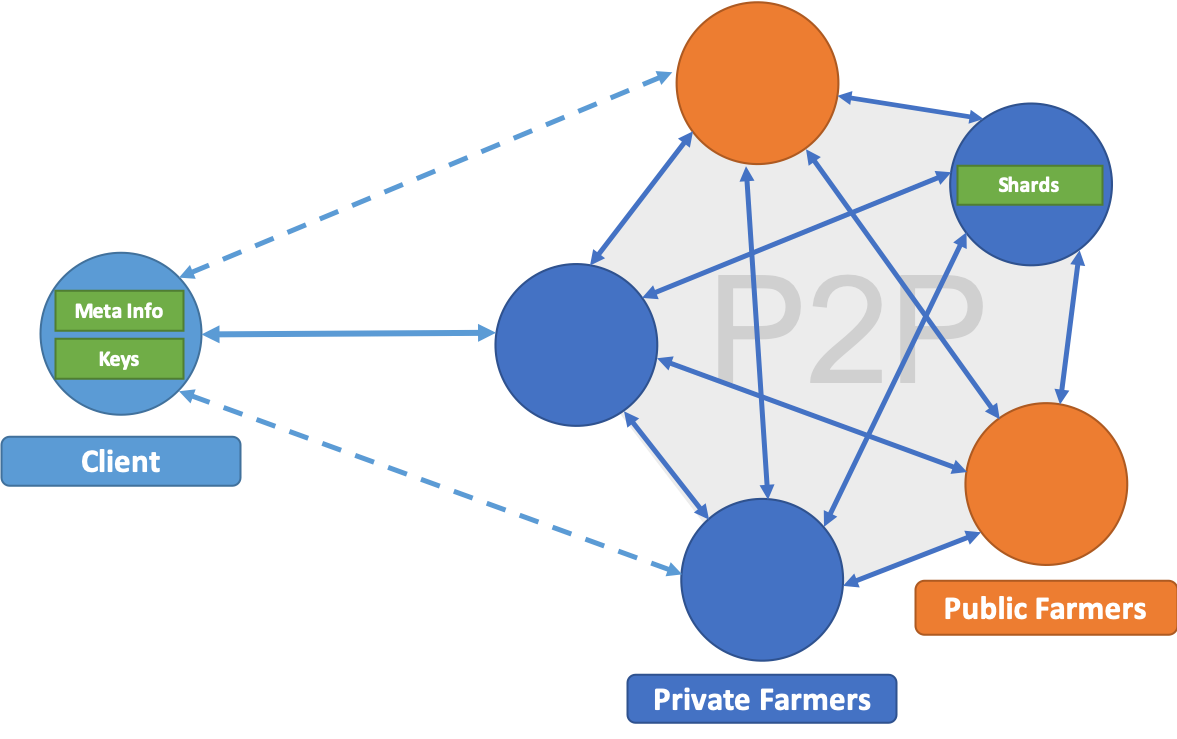
\includegraphics[width=15cm]{figures/system_architecture.png}
  \caption{System architecture}
  \label{fig:systemarchitecture}
\end{figure}

\noindent The FileFarm system is composed of 2 roles:

\begin{enumerate}
  \item \textit{Client}: User-side application providing user interface, handling upload/download tasks and managing file meta along with hash values and encryption keys for later retrieval.
  \item \textit{Farmer}: Basic component of the FileFarm storage network. A farmer is linked with exactly 1 storage provider (either a public cloud or a private data server) to offer storage service. At the same time, farmers connect to each other to form a P2P network and take care of availability of each stored piece of data. A farmer also provides API for clients to store and retrieve data.
\end{enumerate}

As shown in Figure \ref{fig:systemarchitecture}, The FileFarm cloud-of-clouds is formed by farmers, in a sense that service availability has no dependence on any single farmer or its underlying cloud. Thus, FileFarm system has no single-point-of-failure. All farmers provide the same storage service. Thus, client can establish stateless connection with any farmer for uploading/downloading data.

The basic unit of data in FileFarm network is called \textit{shard}, which is a computed segmentation of file that is saved in the network. A specific amount of distinct shards are required to reconstruct the original file, depending on the \textit{sharding schema}. From client's point of view, a file is split, encrypted and then computed into a number of shards with IDA (more details explained in \ref{s:dataconfidentiality}). Instead of the original file, the shards are what actually uploaded. The encryption keys, hashes, file meta are kept by client itself. This ensures that only the client itself is able to reconstruct its own data.

% application models and process flows
\section{Application Models and Process Flows}
\label{s:applicationmodelsandprocessflows}

\begin{figure}[hbt]
\centering
  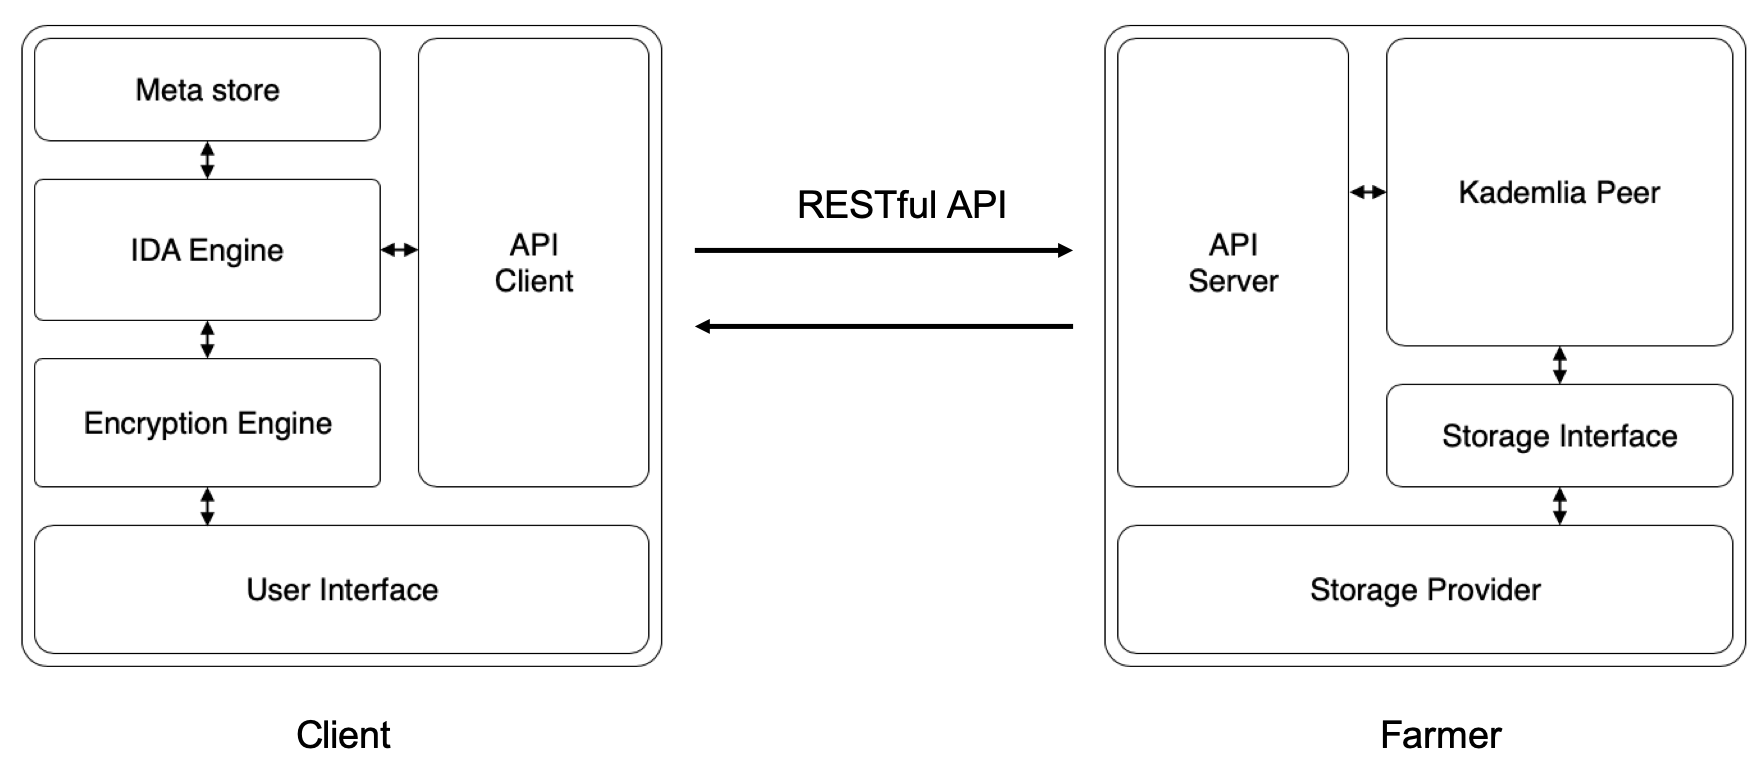
\includegraphics[width=14cm]{figures/application_models.png}
  \caption{Application model of client and farmer}
  \label{fig:applicationmodels}
\end{figure}

Figure \ref{fig:applicationmodels} shows the model of client and farmer applications. Client application has a interface for user to manage their own storage and to upload/download files. When receiving command from user to upload a file, the client application splits the file into slices and pre-process each slice with encryption engine and IDA engine. After pre-process, each slice is transformed into multiple shards, and the encryption keys and hash value of shards are saved in the client's meta store at the same time. The client application then upload each shard to the FileFarm storage network through a randomly-chosen farmer. Farmer application, on the other hand, has a API server module that serves request from client applications. Besides the server module, farmer also has a Kademlia peer module that coordinates with other farmer's corresponding part to synchronize storage status of uploaded shards and provide an efficient way to locate them. In order to apply farmer application on different storage services, FileFarm implements an abstract storage interface layer that provides identical out-bounded API but negotiate with different storage providers according to their API format.

Going with the application model, we present upload / download flow of FileFarm in figure \ref{fig:uploadflow} and figure \ref{fig:downloadflow}, respectively. Some of the processes in these 2 flow diagrams is not clear yet, which will be explained in the following sections.

\begin{figure}[hbt]
\centering
  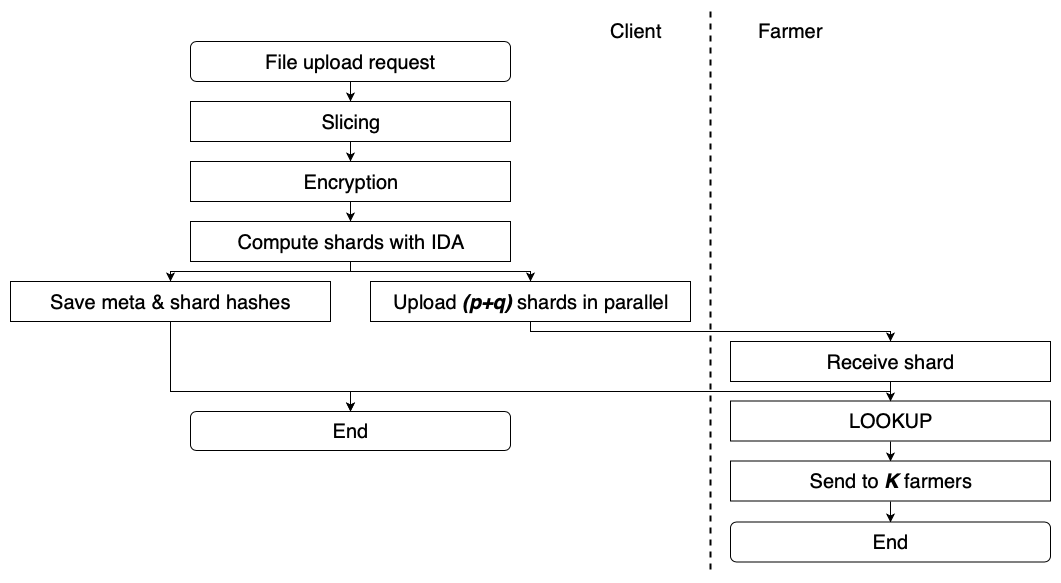
\includegraphics[width=14cm]{figures/upload_flow.png}
  \caption{Upload flow}
  \label{fig:uploadflow}
\end{figure}

\begin{figure}[!b]
\centering
  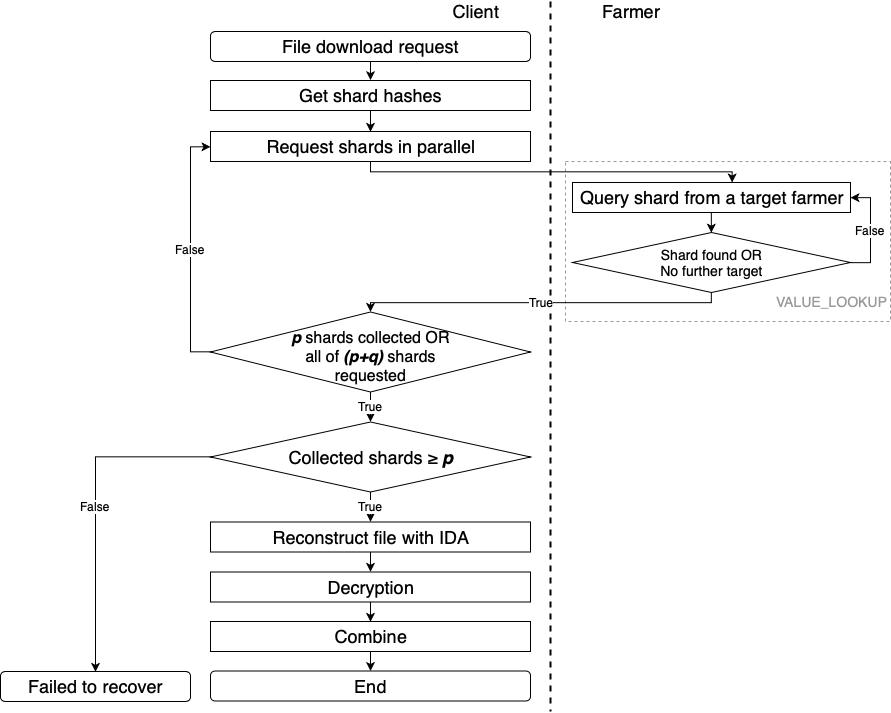
\includegraphics[width=15cm]{figures/download_flow.png}
  \caption{Download flow}
  \label{fig:downloadflow}
\end{figure}

\newpage

% DHT-based approach
\section{DHT-Based Approach}
\label{s:dhtbasedapproach}

To find shards in a P2P network, FileFarm implements Kademlia DHT protocol. As described in \ref{s:kademlia}, Kademlia protocol gives FileFarm benefits in the following aspects:

\begin{enumerate}
  \item \textit{Load balancing}: storage load of each farmer is roughly balanced.
  \item \textit{Efficient search}: lookups in FileFarm needs no more than logarithm steps.
  \item \textit{Redundancy maintenance}: each shard will always be stored on at least $K$ farmers.
\end{enumerate}

Instead of saving location of shards as static records in a centralized database, FileFarm adopts Kademlia's dynamical lookup procedures. Before storing a shard, a farmer uses the NODE\_LOOKUP procedure to determine on which farmers the shard should be stored, and then send parallel storing messages to these farmers. In the case of shard retrieval (download), a farmer performs VALUE\_LOOKUP procedure to find the shard iteratively until it is found. Both NODE\_LOOKUP and VALUE\_LOOKUP procedures are robust to churn of farmers, network topology changes and scaling of network size, which usually can not be handled well in centralized solutions. Besides, since given shard, the $K$ farmers to store it are uniquely defined and the results of NODE\_LOOKUP and VALUE\_LOOKUP procedures have no dependence on originating node, a client can request any farmer to upload or download the shard, which will eventually be stored on the same set of farmers. This allows a parallel and fault-tolerant design in which clients can upload /download different shards from different farmers simultaneously and do not rely on a specific farmer to perform these tasks.

% Beyond Kademlia
\section{Beyond Kademlia}
\label{s:beyondkademlia}

From \ref{s:dhtbasedapproach}, we acknowledged that FileFarm inherits a number of benefits from Kademlia. However, Kademlia was originally invented for content-sharing applications but not storage systems. To claim FileFarm as an enterprise storage, we also need to consider following requirements that cannot be provided by Kademlia:

\begin{enumerate}
  \item \textit{Data confidentiality}
  \item \textit{Access management}
  \item \textit{Cost efficiency}
  \item \textit{Retrievability}
\end{enumerate}

\noindent Corresponding mechanisms are designed to meet these requirements:

\begin{enumerate}
  \item \textit{Encryption and information dispersal algorithm}
  \item \textit{Decentralized authentication}
  \item \textit{Storage release and prioritized download}
  \item \textit{Public farmer ID assignment}
\end{enumerate}

\noindent These mechanisms will be explained in the following sections \ref{s:dataconfidentiality}, \ref{s:accessmanagement}, \ref{s:costefficiency}, \ref{s:retrievability}.

\begin{figure}[hbt]
\centering
  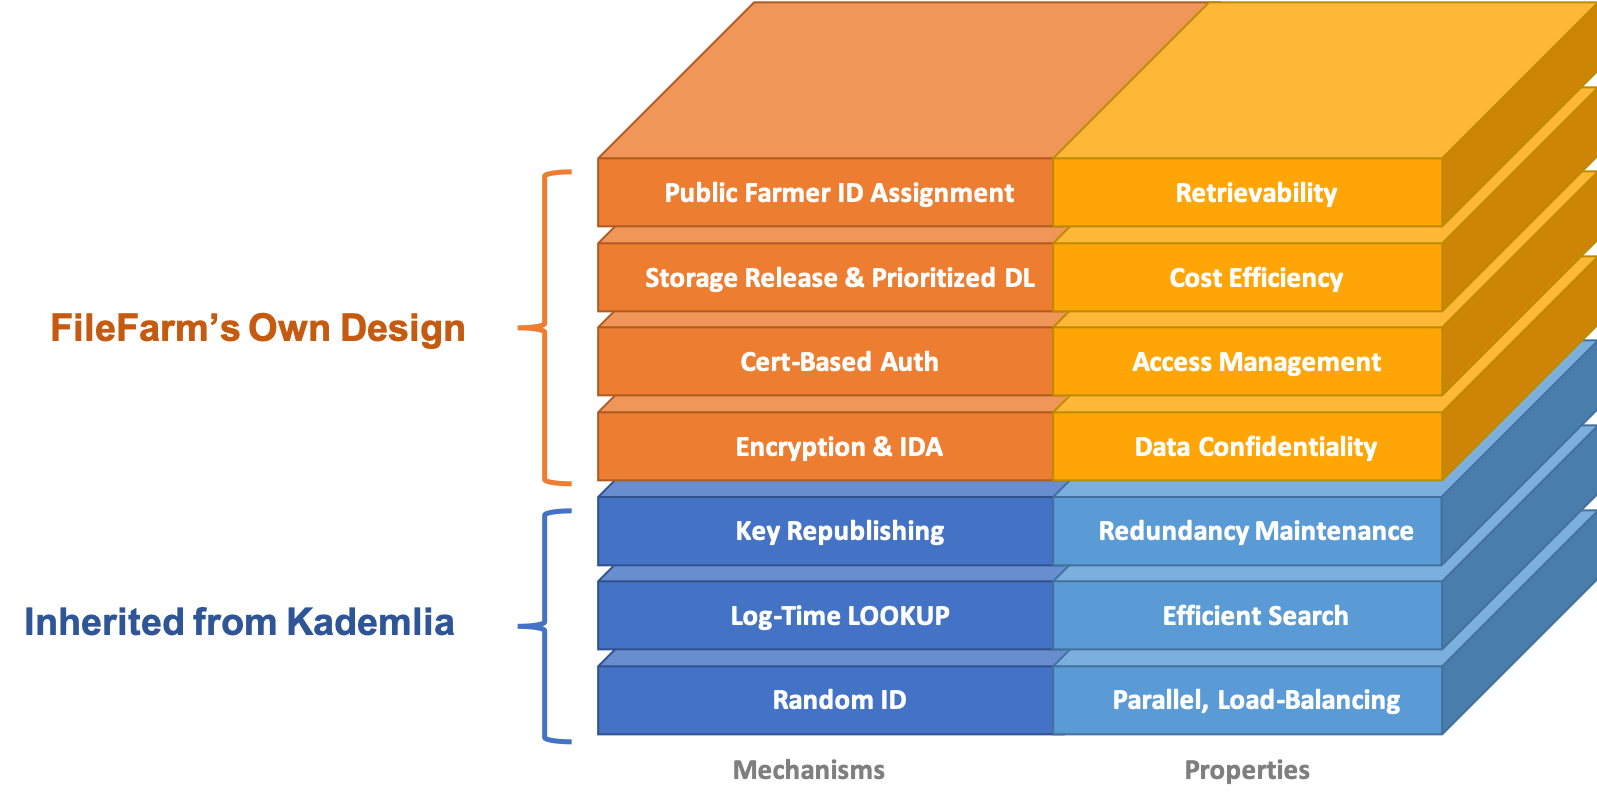
\includegraphics[width=14cm]{figures/property_stack.png}
  \caption{FileFarm's property stack}
  \label{fig:propertystack}
\end{figure}

% data confidentiality
\section{Data Confidentiality}
\label{s:dataconfidentiality}

Designed to be a general-purposed P2P content sharing overlay, vanilla Kademlia protocol does not provide features of encryption and dispersion since data are meant to be shared instead of being kept in secret in most P2P applications. Thus, without confidentiality design, files will be uploaded to Kademlia network directly and the storing nodes will be able to peek content of the files. However, as FileFarm is a private storage system targeting on preserving data security and privacy, the mechanisms considering data confidentiality must be designed.

In order to preserve privacy and confidentiality while storing data on public clouds, FileFarm introduces a pre-processing flow of files before they are actually uploaded, in a sense that every files are randomly dispersed over clouds, and only the owner holds the key to retrieving and reconstructing them. To be precise, an example is shown in Figure \ref{fig:dataconfidentiality}. A file $F$ of size $S$ is sliced into chunks $C1, C2, ..., Cn$ of size $\frac{S}{n}$ and then chunks are encrypted into $E1, E2, ..., En$ of the same size, respectively. For each of the encrypted chunk, a \textit{sharding} process is performed based on an Information Dispersal Algorithm of $(p,q)$ schema (see \ref{s:informationdispersalalgorithm}), which produces $(p + q)$ shards of size $\frac{S}{n}*\frac{p+q}{p}$, and the original encrypted chunk can be recovered from any $p$ of these $p + q$ shards. Now the pre-processing flow is finished, and the $n * (p + q)$ generated shards are uploaded to FileFarm in parallel.

\begin{figure}[!b]
  \centering
    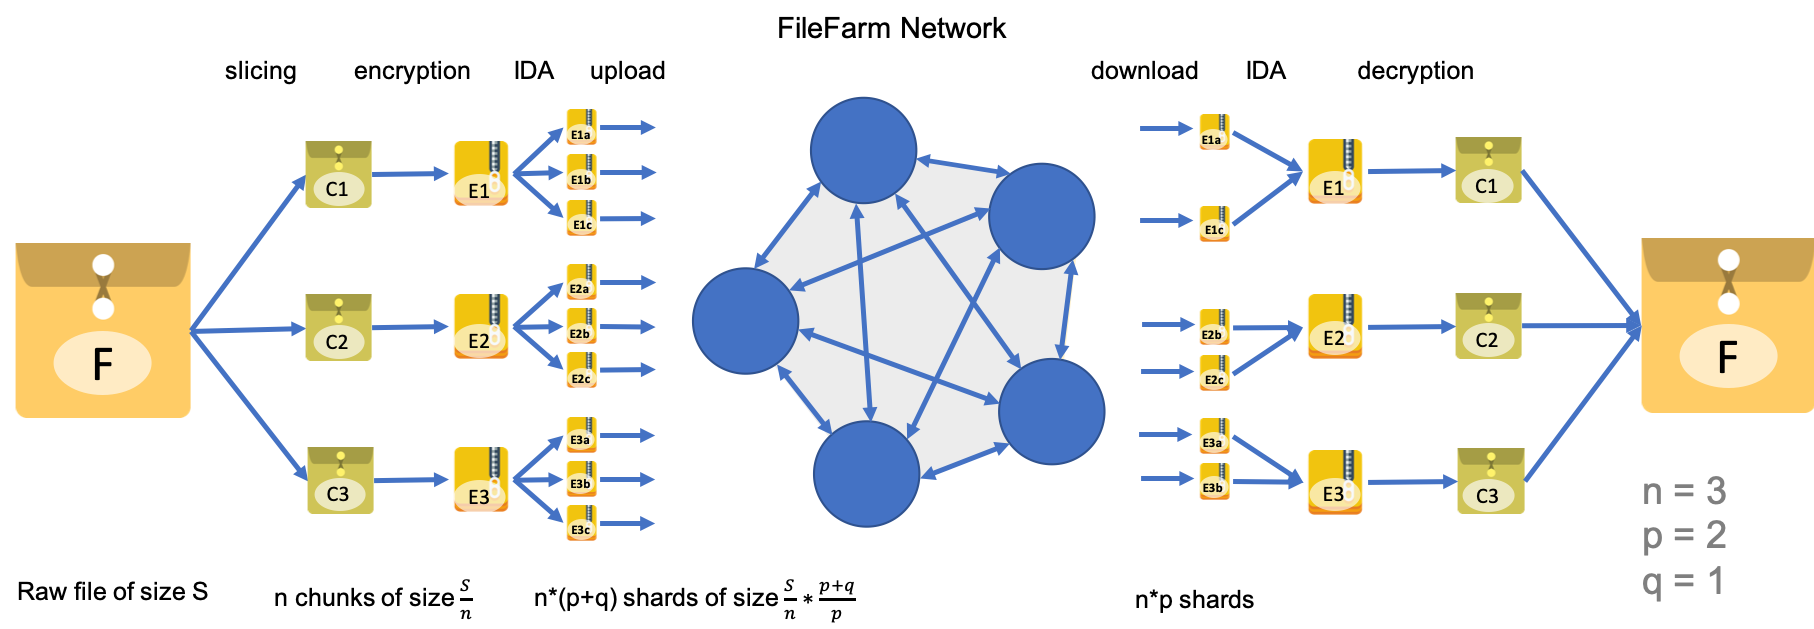
\includegraphics[width=15cm]{figures/data_confidentiality.png}
    \caption{An example of encryption and sharding flow}
    \label{fig:dataconfidentiality}
\end{figure}

To reconstruct the original file $F$, the procedure seems inverted. For each of the encrypted chunks $E1, E2, ..., En$ that was sharded into $p+q$ shards, the client sends parallel requests to collect $p$ shards so that it can be reconstructed by IDA. The reconstructed chunks are then decrypted to $C1, C2, ..., Cn$ and combined into the original file, $F$.

% access management
\section{Access Management}
\label{s:accessmanagement}

Different from general P2P applications, FileFarm is an enterprise storage system applied in a \textbf{private} context. In such usage scenario, how to grant access to authorized users while denying connections from unauthorized ones plays a crucial role in security of the system. To achieve this goal, FileFarm adopts a decentralized approach toward access management. Different from common web systems, the access management design in FileFarm does not involve a centralized key directory. Instead, the account and key information is saved distributed-ly in FileFarm storage network, just like normal data, which means the access management mechanism has no dependence on any single farmer, and no data leakage will occur even if any farmer is compromised.

\subsection{Decentralized Authentication}
\label{ss:decentralizedauthentication}

The decentralized authentication mechanism involves 2 major parts: (1) \textit{register}, (2) \textit{login}.

\begin{enumerate}
  \item \textbf{Register}: This process occurs when a user accesses the FileFarm system for the first time. From user's point of view, the goal of this process is to create an account, get permission from the administrator and then save account information into the network so that it can be accessed successfully next time, probably from a different client machine. This approach is based on the concept of Public Key Infrastructure, which is described in \ref{s:publickeyinfrastructure}, whereas the goal here is to validate clients but not serving hosts. The approach involves 3 roles: an administrator, the FileFarm cloud, and a user accessing FileFarm through a client application. To register an account, the user determines an account name($Account_{U}$) and a password ($Passwd_{U}$) in the client application. The account name and password will be hashed into user ID ($ID_{U}$) and private key ($PriKey_{U}$), respectively. The client application then checks existence of the account name by querying from the FileFarm cloud with user ID. If the account has not been registered yet, the procedure goes on. Client application will wrap (1) account name, (2) user ID, (3) user information, (4) a public key ($PubKey_{U}$) generated from user's private key and (5) a user's signature ($Sig_{U}$) into a certificate request (CSR). On receiving such request, the administrator makes a decision on whether to grant access for the client or not. If the client passes administrator's validation, the administrator creates a signature ($Sig_{A}$) on the signing request, which turns into a certificate. The certificate is then sent back to the client. When receiving a valid certificate, the client application stores it on the FileFarm cloud with key being her user ID, and the registration process is finished successfully.

  \item \textbf{Login}: This process is designed for a registered user to login to his account with account name and password, which are the only information needed to be carried by the user. The user can login via a client machine different from the one he used to register account. To login to FileFarm, the user first types account name ($Account_{U}$) and password ($Passwd_{U}$) into the client interface. The account name and password are hashed into user ID ($ID_{U}$) and private key ($PriKey_{U}$), respectively. Then the client application makes a query for the user's certificate from the FileFarm cloud. On receiving the certificate, the client verifies user's password by checking the signature on it. If the password validation succeeds, the client is allowed to access the FileFarm storage network. To access FileFarm, the client appends its certificate to the connection request packet, and then encrypts the payload with its own private key. When receiving request from clients, a farmer check the validity of the certificate by verifying the signature on it using administrator's public key. The farmer also verifies client's identity by decrypting the payload using client's public key specified in the certificate.
\end{enumerate}

\begin{figure}[hbt]
  \centering
    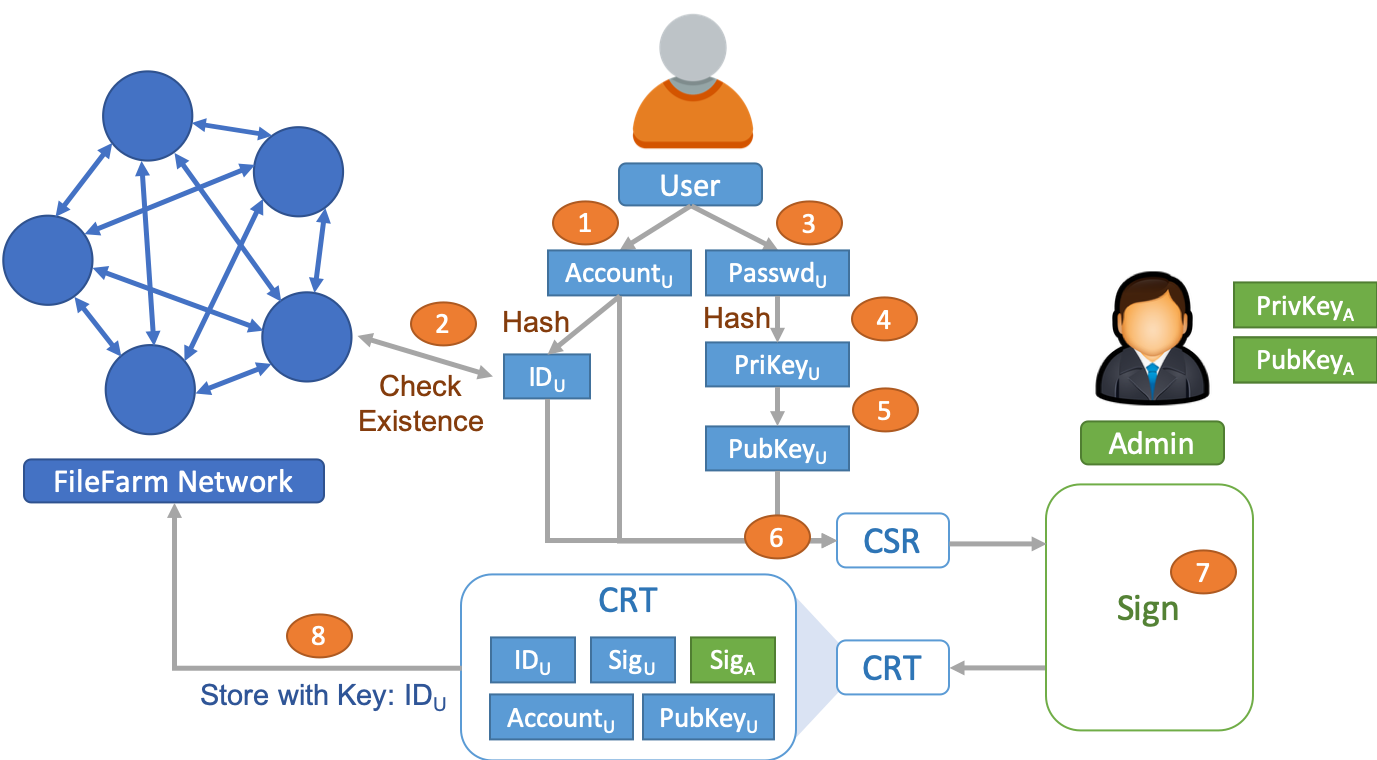
\includegraphics[width=14cm]{figures/access_management_register.png}
    \caption{An illustration of register procedure}
    \label{fig:accessmanagementregister}
\end{figure}
  
\begin{figure}[!b]
  \centering
    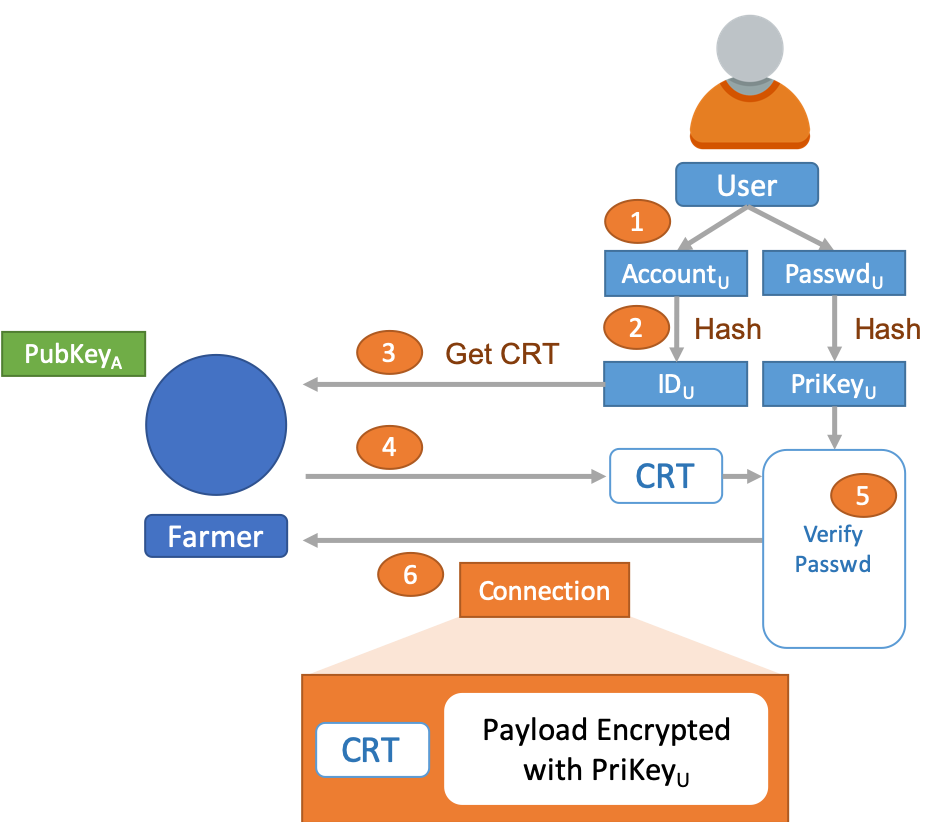
\includegraphics[width=12cm]{figures/access_management_login.png}
    \caption{An illustration of login procedure}
    \label{fig:accessmanagementlogin}
\end{figure}

\newpage\phantom{blabla}
\newpage\phantom{blabla}

% cost efficiency
\section{Cost Efficiency}
\label{s:costefficiency}

FileFarm is built on the top of both public clouds and private premises. Storage fees are charged by public storage provider but not by the enterprises' own servers. Due to this fact, any storage operation executed on public clouds needs to be carefully inspected, in order to minimize the fee charged by public storage providers without lost of retrievability. As depicted in \ref{table:cloudstoragecost}, there are 2 major kind of storage fees: (1) \textit{static storage fee} per-GB / per-month (2) \textit{data transfer out fee} per-GB of download traffic. We will explain how the redundant fee comes from the original design and introduce the mechanism employed by FileFarm to reduce these fees in the following sub-sections.

\subsection{Storage Release}
\label{ss:storagerelease}

The \textit{storage release} mechanism reduces \textit{static storage fee} by releasing unused redundant copies of shard and keeping redundancy at \textit{exactly K} but not more. To understand why there might be unused redundant copies of shard, we need to take a look at how the underlying Kademlia DHT protocol maintains redundancy.

As described in \ref{ss:redundancymaintenance}, Kademlia implements an \textit{Efficient Key Republishing} mechanism that ensures each shard will always have "at least" $K$ copies over the storage network. However, there are certain scenarios making number of copies more than $K$, which results in unneeded storage overhead. Considering a scenario in which a shard is kept by $K$ farmers and one of them churns off accidentally. With efficient key republishing, one of the remaining $K-1$
farmers will detect this and send a copy of the shard to the $K+1^{th}$ closest farmer, so that redundancy recovers from $K-1$ to $K$. However, when the failed farmer recovers from service outage, the redundancy will raise from $K$ to $K+1$. The copy on the $K+1^{th}$ closest farmer is now an unused overhead that need to be eliminated in order to save static storage cost.

This is the moment that storage release mechanism should work. Due to the fact that republishing message will only be sent to the $K$ closest farmers, the $K+1^{th}$ closest farmer will not receive this message, which triggers it to republish the shard in the next period. To find the $K$ closest farmers to this shard, a NODE\_LOOKUP procedure should be performed before sending republishing messages. This gives the $K+1^{th}$ closest farmer a chance to find itself not being one of the K closest farmers, it then stops the republishing process and deletes the shard from its storage. This shows the entire working procedure for storage release mechanism.

From the explanation above, we make a brief conclusion that \textit{storage release} is a mechanism that minimizes \textit{static storage fee} by holding redundant copies of each shard at exactly $K$ but not more. Besides, as the $K$-redundancy guideline still holds, \textit{storage release} does not induce retrievability concerns.

\subsection{Prioritized Download}
\label{ss:prioritizeddownload}

\textit{Prioritized download} is a mechanism aiming to minimize the \textit{data transfer out} fee from public clouds. This mechanism only makes sense in hybrid cloud settings, where not only public clouds but also enterprise's private storage machines such as NAS or SAN are contributed to the storage system. Without \textit{prioritized download} mechanism, each farmer is treated equal and shares the same probability of serving data for clients. However, the cost of downloading data from public clouds is significantly higher than that of downloading from private servers, because of the \textit{data transfer out fee} charged by storage providers. \textit{Prioritized download} is the mechanism ensuring that shards are preferred to be downloaded from private farmers, so that \textit{data transfer out fee} is minimized.

In hybrid-cloud settings, enterprises optionally build their own private farmers. The private farmers are usually not as reliable as public ones. However, they have advantages in at least 2 aspects:

\begin{enumerate}
  \item High throughput and low delay in local area network (LAN)
  \item No data transfer fee needed
\end{enumerate}

These advantages make it reasonable for enterprises to split a portion of budgets on investment of private storage devices. This not only reduces data transfer fee charged by public clouds, but also improves download performance.

To understand how prioritized download works, we need to take a closer look at how the underlying Kademlia DHT protocol retrieves a shard. As described in \ref{ss:efficientsearch}, Kademlia implements an iterative VALUE\_LOOKUP procedure to retrieve shards. The VALUE\_LOOKUP procedure finishes immediately when any of the visiting farmers does store the shard, and the client will download the shard from that farmer.

Prioritized download is a modified version of VALUE\_LOOKUP, with some noticeable differences:

\begin{enumerate}
  \item Prioritized download finishes once the target shard is found on a \textbf{private} farmer.
  \item Prioritized download memorizes a public farmer who has the shard when finding such one, but not download from it immediately.
  \item Prioritized download downloads from a public farmer only if there is no private farmer found storing the target shard
\end{enumerate}

By applying these differences to the VALUE\_LOOKUP procedure, \textit{prioritized download} ensures that shards will be downloaded from public farmers only if there is no private farmer serving the same shard. This effectively minimizes the data traffic flowing out from public clouds and also the \textit{data transfer out fee} charged by storage providers. Since \textit{prioritized download} only changes the preference of downloading order, any public farmer serving the shard will eventually be chosen once there are no private farmers serving the same shard. This implies that \textit{prioritized download} does not affect retrievability of files.

From the description above, we know that FileFarm treats public farmers and private farmers differently. In fact, a special approach is implemented by FileFarm to achieve this kind of differentiation. We will explain the details and the benefits brought by such differentiation in \ref{ss:publicfarmeridassignment}.

% retrievability
\section{Retrievability}
\label{s:retrievability}

In FileFarm's design, redundancy introduced by the $K$ factor of Kademlia (\ref{s:kademlia}) and the $q$ factor of information dispersal algorithm (\ref{s:informationdispersalalgorithm}) both contribute to retrievability of files. However, considering a hybrid-cloud case in which some shards are stored totally on private farmers but no public ones. The significant reliability difference between public and private farmers would cause a large disparity in retrievability of files, which makes the system's behavior unpredictable. To provide a more rigorous guarantee on retrievability in hybrid-cloud settings where reliability of public clouds and private servers differs greatly, we have to make sure every shard is saved on at least 1 public cloud with high probability. This demand gives rise to the design of \textit{public farmer ID assignment}.

\subsection{Public Farmer ID Assignment}
\label{ss:publicfarmeridassignment}

To differentiate public farmers from private ones, FileFarm gives public farmers a special identity. In the 160-bit farmer ID space, each public farmer is assigned with an ID with last 144 bits be '0', hence there can be at most $2^{16}=65536$ public farmers in the network. In contrast, ID of private farmers are generated randomly but cannot have last 144 bits be '0'. Besides, public farmer IDs are issued in bit-reversal permutation ordering. To be clear, we explain this kind of ordering in a simplified case where public IDs vary in the first 4 bits and have last 156 bits be '0' (see figure \ref{fig:bitreversalpermutationordering}). To generate ID for the $i^{th}$ public farmer, we reverse the binary representation of the number $i-1$ and assign the resulting binary string as the first 4 bits of the newly-generated ID. Following this rule, the first 4 bits of generated public IDs will be '0000', '1000', '0100', '1100', ...

With public farmer IDs being assigned in bit-reversal permutation ordering, we can be certain that public farmers are dispersed over the 160-bit ID space. Since that hash value of shards follow a uniform distribution over the 160-bit key space and that shards are stored on farmers with ID closest to its hash value, the dispersion of public farmer IDs makes them load-balanced in terms of storage usage and request frequencies. Besides, this explicit assignment also avoids the situation that public farmer's IDs distribute uneven over the network, which would cause disparity between retrievability of shards.

To sum up, the assigning rule of public farmer ID brings following benefits:

\begin{enumerate}
  \item Provides an explicit rule to distinguish public farmers from private ones, which is needed for prioritized download (\ref{ss:prioritizeddownload}) to work.
  \item Poses a strong guarantee on load-balancing of public farmers, which in further minimizes the reliance on any single public cloud.
  \item Maximizes the likelihood of each shard to be stored by at least one public farmer, which improves the average retrievability of each shard and thus enhances the overall retrievability of files.
\end{enumerate}

\begin{figure}[!b]
\centering
  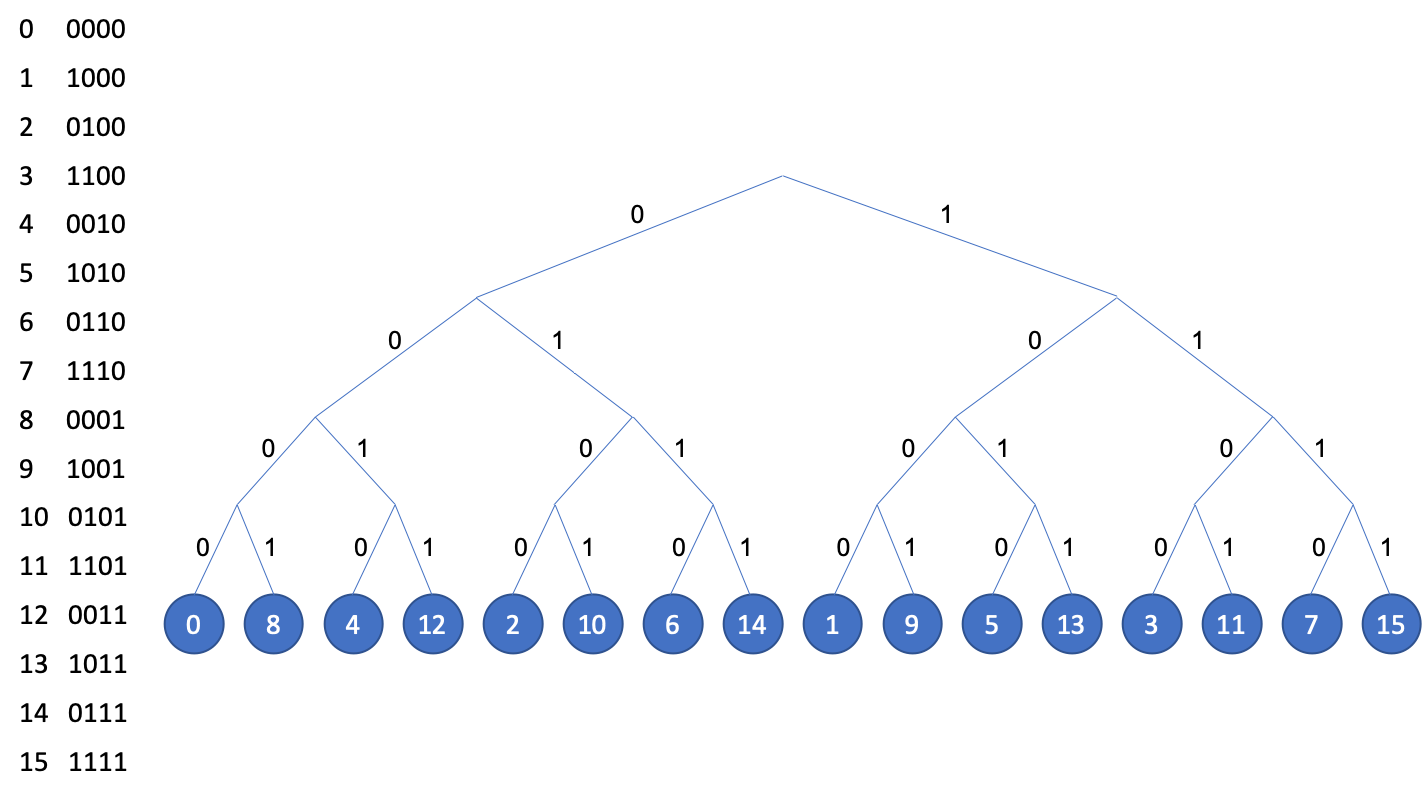
\includegraphics[width=15cm]{figures/bit_reversal_permutation_ordering.png}
  \caption{Bit-reversal permutation ordering with prefix length = 4}
  \label{fig:bitreversalpermutationordering}
\end{figure}